\clearpage
\twocolumn[{%
\subsection{Agreement with DataDecide}
\label{app:rq07_external_frameworks}

\noindent\begin{minipage}[t]{0.485\textwidth}
\vspace{0pt}
\paragraph{Research Question.} \emph{Do the SNR variants and the ``reliable benchmark'' set we find on our ladder also hold on AllenAI's DataDecide / OLMo corpus, on the English benchmarks both share?}

\paragraph{Setup.} We compare our 1B rung (seed 1904, every cell and data build) with the 1B rung of DataDecide (25 data recipes). We use the English tasks that both evaluate and that clear the above-chance gate on our side. SNR is the average absolute deviation over noise, and we compare it on a log scale.
\end{minipage}\hfill
\begin{minipage}[t]{0.485\textwidth}
\vspace{0pt}
\begin{rqfinding}
\textbf{1. Both corpora rank the three gated shared tasks the same way (ARC Easy $>$ HellaSwag $>$ ARC Challenge, Spearman $\rho$ 1.00, Pearson r of log$_{10}$ SNR 0.87, p = 0.33).} But three points are too few for the agreement to be evidence. (Figure~\ref{fig:app_rq07_external_frameworks}.)
\\
\\
\textbf{2. Same order, n = 3.} \texttt{aad} SNR is 1.03 / 0.82 / 0.50 on our ladder and 9.76 / 5.04 / 4.16 on DataDecide for ARC Easy / HellaSwag / ARC Challenge.
\\
\\
\textbf{3. Our SNR is 6.1--9.4$\times$ smaller.} DataDecide's \texttt{aad} SNR exceeds ours by 9.4$\times$ on ARC Easy, 6.1$\times$ on HellaSwag and 8.2$\times$ on ARC Challenge. The log-scale correlation ignores this offset, so compare orders across corpora, never SNR levels.
\end{rqfinding}
\end{minipage}

\vspace{\baselineskip}
\noindent\begin{minipage}{\textwidth}
\centering
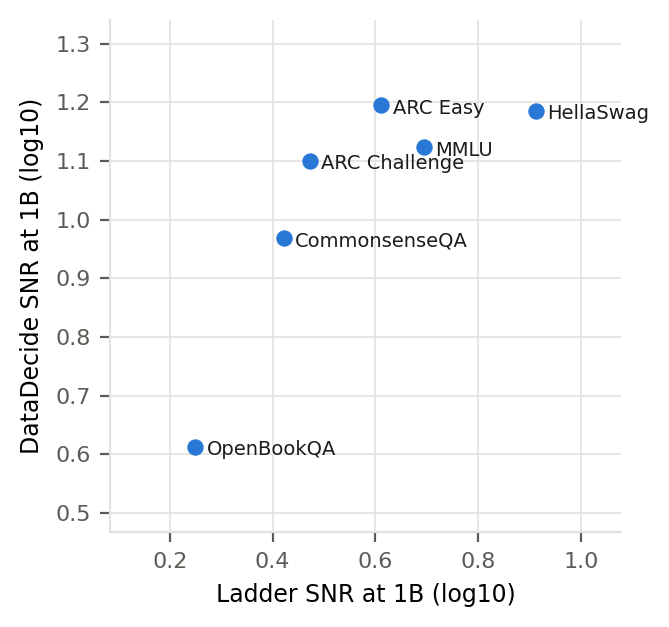
\includegraphics[width=\textwidth,height=0.4\textheight,keepaspectratio]{figures/app_rq07_external_frameworks.png}
% source: src/signal-and-noise/analysis/rq07_external_frameworks/pretraining/predictivity/snr_apertus_vs_snr_allenai_paper.png
\captionof{figure}{\textbf{Both corpora rank the three gated shared tasks the same way (ARC Easy $>$ HellaSwag $>$ ARC Challenge, Spearman $\rho$ 1.00, Pearson r of log$_{10}$ SNR 0.87, p = 0.33).} Each point is one English task that both our ladder and DataDecide evaluate and that clears the above-chance gate on our side. The x axis gives the SNR of our 1B rung and the y axis the SNR of the DataDecide 1B rung, both on a log10 scale.}
\label{fig:app_rq07_external_frameworks}
\end{minipage}
\vspace{\baselineskip}
}]
